\documentclass{article}
\usepackage[utf8]{inputenc}
\usepackage{multirow}
\usepackage{verbatim}
\usepackage[pdftex]{graphicx}
\usepackage{subfigure}


\begin{document}
\title{Profiling users media preferences based on social network data streams}
\author{Konrad Delong \and Antoni Piechnik}
\date{May 25 2010}

\maketitle

\begin{abstract} Social networks have been becoming hugely popular over the last
years. With enormous number of people sharing information about their lives,
they are now a great source of information about their interests. Based on both
structured data (such as the social aspect of YouTube) as well as unstructured
(Twitter), we will be trying to find out how accurately we can profile user's
preferences for it to be usable in a real life project (NoTube).
\end{abstract}

\section{Problem statement}
The NoTube project bases its recommendation on aggregating, extracting and analyzing user activities. Since media oriented web services (such as YouTube) hold a great amount of information regarding a users' video viewing preferences, it might provide a great deal of additional information for profiling NoTube users. General activity services (social networks like Facebook or Twitter) detail the lives of its users, it is very likely that they also contain information regarding their tv watching activities.

The most important question is what user data we can collect from both structured and unstructured social applications? When it comes to YouTube, users can mark videos as favorite, subscribe to other users' channels and comment on videos. From all that information we can not only extract the titles of videos they are interested in but also tags describing them as well as relations to other videos. On the other hand, unstructured data streams like Twitter contain much more irrelevant information, but can enable us to extract a greater amount of activities limited only by what the natural language offers. Apart from extracting the activities, we will be able to relate the entities (like TV programme and channel names). A user profile could also be partially generated from a user's activity frequency as well as the users they are following and the hash tags used.

Another part of the project will cover finding ways of measuring the accuracy and effectiveness of profiling a user based on those social data streams. We would like to find out how efficient browsing through different networks is when it comes to generating those profiles, both in terms of the quality of information regarding the media preferences as well as its amount relative to the amount of data collected. We will attempt to find a perfect ratio between the level of detail of the information we extract and the quality of user profiles generated. We will evaluate interest counting strategies for different types of entities recognized in various contexts.  

\section{Draft plan of work for the Twitter/Youtube project}

\subsection{16.03.2010}
\begin{itemize}
\item{Creating data scrapers for collecting data}
\item{Research into entity recognition papers (if applicable)}
\item{Begin implementing the data extraction algorithms}
\end{itemize}

\subsection{23.03.2010}
\begin{itemize}
\item{Initial results presentation.}
\item{Discussing used methods and possibilites of improving their results.}
\end{itemize}

\subsection{30.03.2010/06.04.2010}
\begin{itemize}
\item{Presenting the results of the improved methods for extracting data
from Twitter and YouTube separately.}
\end{itemize}

\subsection{13.04.2010}
\begin{itemize}
\item{Implementing tubelets (merging our implementations with the Beancounter)}
\item{Start working on the first deliverable (by comparing our results)}
\end{itemize}

\subsection{20.04.2010}
The draft of the Deliverable 1:
A comparative analysis of Twitter and Youtube streams as sources of data
regarding Art and TV preferences of their users.


\subsection{27.04.2010}
\begin{itemize}
\item{Research of various counting methods used both by NoTube as well as on
external cases (if any)}
\item{Discussing the possible use of- and choosing the methods for counting
purposes.}
\end{itemize}

\subsection{04.05.2010}
\begin{itemize}
\item{Implementing the chosen methods}
\item{Measuring effectiveness.}
\item{Initial results presentation.}
\end{itemize}

\subsection{11.05.2010}
\begin{itemize}
\item{Merging our implementations with the Beancounter (Reasonlets)}
\item{Measuring the influence of enrichment approaches on the efficiency of profile
generation methods.}
\item{Beginning work on the second deliverable.}
\end{itemize}

\subsection{18.05.2010}
The draft of the Deliverable 2:
What are the counting strategies, how can we improve them using different
enrichment methods?


\subsection{25.05.2010}
\begin{itemize}
\item{Working on the deliverables, taking the Notube team's comments and suggestions
into consideration.}
\end{itemize}


\subsection{01-15.06.2010}
\begin{itemize}
\item{Improving results of the taken approaches for both deliverables based on an
increasing amount of data collected.}
\item{Working on the final paper}
\end{itemize}

\newpage
\section{YouTube}

\subsection{YouTube information}

\begin{tabular}{l p{3cm} l p{4cm}}
Concerning & Information & Access & Description\\ \hline
Video & Title & Public API \\
Video & Published & Public API \\
Video & Updated & Public API \\
Video & Category & Public API \\
Video & Tags (keywords) & Public API \\
Video & Comments & Public API \\
Video & Permissons & Public API \\
Video & Description & Public API \\
Video & Thumbnails & Public API & Set of video's thumbnails (along with times
when taken) \\
Video & Duration & Public API \\
Video & Ratings & Public API & Best, worst and average rating, number of votes
\\
Video & Viewcount & Public API \\
Video & Favourite count & Public API \\
Video & Number of likes & Public API \\
Video & Number of dislikes & Public API \\
Video & Aspect ratio & Public API \\
Video & Related & Public API \\
Video & Responses & Public API \\
Video & Author & Public API \\

Video search & Number of results & Public API \\
Video search & Search results & Public API \\

User & Uploads & Public API \\
User & Gender & Public API \\
User & Location & Public API \\
User & Age & Public API \\
User & Contacts & Public API \\
User & Username & Public API \\
User & Subscriptions & Public API \\
User & Inbox & Public API \\
User & Favorites & Public API \\

Comment & Created & Public API \\
Comment & Updated & Public API \\
Comment & Author & Public API \\
Comment & Text & Public API \\

User's channel & Demographics (viewers' age/gender) & Screen scraping \\
User's channel & Referrers & Screen scraping \\
User's channel & Popularity across countries & Screen scraping \\
User & History & Screen scraping \\
User & Likes & Screen scraping \\
User & Issued authentication subtokens & Screen scraping \\

Video & Subtitles & OCR \\

\end{tabular}

\subsubsection{YouTube usage}

A statistics were performed measuring popularity of three YouTube features: favourites,
subscriptions and uploads. Over a sample of 7500 users most settled down at
relatively low level of activity. All histograms below show numbers of users
(axis y) with $x_1-x_2$ numbers of favourites/subscriptions/uploads. The
logarithmic scale was used for all three charts.

\begin{figure}[ht]
\centering
\subfigure[Favourites]{
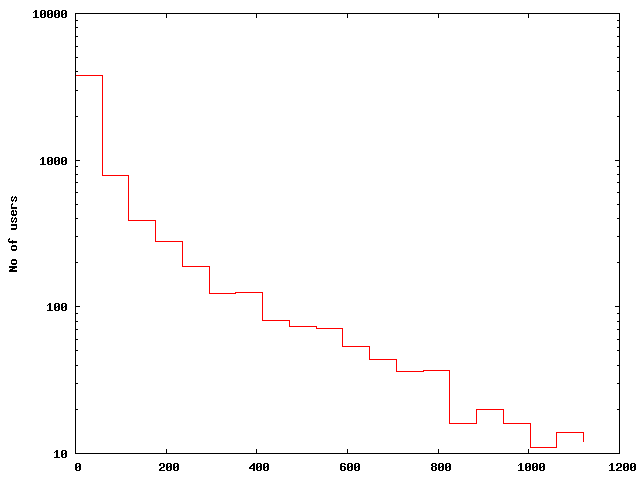
\includegraphics[scale=0.6]{images/favs.png}
\label{fig:favs}
}
\subfigure[Subscriptions]{
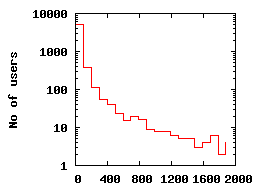
\includegraphics[scale=0.6]{images/subs.png}
\label{fig:subs}
}
\subfigure[Uploads]{
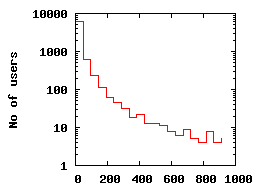
\includegraphics[scale=0.6]{images/ups.png}
\label{fig:ups}
}
\label{fig:subfigureExample}
\caption{Histograms of usage of favourites \subref{fig:favs}, subscriptions
\subref{fig:subs} and uploads \subref{fig:ups}. The x axis represents groups of
users having $x_1-x_2$ entities, the height of the bars indicates sizes of the
groups.}
\end{figure}

\subsubsection{YouTube counting strategies}

\begin{itemize}
\item{Tags aggregation across various video sets:
\begin{itemize}
  \item{User's likes and favourites}
  \item{User's subscriptions (two-level aggregation there)}
  \item{User's history}
  \item{User's uploads}
\end{itemize}
}

\item{Similar aggregation for other entities found in videos
\begin{itemize}
  \item{Puropose of the video -- we could invent a dictionary of video purposes
  (eg. advertisements, lectures, speeches, movie fragments, family videos) and
  relate them to the videos.}
  \item{Keywords from comments -- after the aggregation and rejecting of stop
  words, this might prove userful.}
  \item{Language -- could be estimated by analysis of language of
  comments and description, location of the publisher and commenters.}
  \item{Duration -- users might prefer shorter clips. This might happen only for
  certain types of videos (lectures, advertisements).}
  \item{Freshness -- users might prefer videos uploaded more recently. This
  might be useful for example to identify "sneak peeks" for TV shows.}
  \item{Controversiality -- likes/dislikes ratio, amount of favourites per
  views.}
  \item{Second order effects -- facts determined for a video might be applicable
  also for a clip it is a response to.}
\end{itemize}
}

\item{Relating videos and channels to entities from other linked data services
\begin{itemize}
  \item{People: music artists, actors, directors, politicians, TV presenters,
  other public figures}
  \item{Places: cities, countries}
  \item{Existing works: TV programmes, movies, music tracks}
  \item{Others: musical, political, traditional and commercial events, brands}
\end{itemize}
}
\end{itemize}

\subsection{Counting YouTube tags and categories}
The most obvious way to get profiling information is through the use of
tags. However, tags of a single video clip can be either too numerous, making many
of them irrelevant, too sparse, nonexistent and occasionally just wrong. To avoid
that problem, we aggregate the tags across sets of video clips related to the
profiled user (favourites, subscriptions, uploads). Similar aggregation was
performed for the videos' categories. Below is a comparison of results of counting
tags (chosen by the user) and categories (picked from a small predefined set).







\begin{table}[ht]
\begin{minipage}[b]{0.5\linewidth}\centering

\begin{tabular}{| l | l |}
Category & \# \\ \hline
News & 8 \\
Music & 5 \\
Education & 3 \\
Comedy & 2 \\
\end{tabular}

\end{minipage}
\hspace{0.5cm}
\begin{minipage}[b]{0.5\linewidth}
\centering

\begin{tabular}{| l | l |}
Tag & \# \\ \hline
sonik & 5 \\
bogusław & 5 \\
trzech & 5 \\
kupli & 5 \\
wybory & 4 \\
kraków & 4 \\
polska & 4 \\
\end{tabular}

\end{minipage}

\caption{Most popular tags and categories from account of Bogusław Sonik -- a
polish politician. The word ''wybory'' stands for ''election'' in polish, and
\emph{Trzech kumpli} is a title of a controversial political documentary.}
\end{table}


\begin{table}
\begin{minipage}[b]{0.5\linewidth}\centering

\begin{tabular}{| l | l |}
Category & \# \\
Music & 53 \\
Comedy & 20 \\
Entertainment & 8 \\
Games & 4 \\
People & 3 \\
Travel & 3 \\
News & 2 \\
\end{tabular}

\end{minipage}
\hspace{0.5cm}
\begin{minipage}[b]{0.5\linewidth}
\centering

\begin{tabular}{| l | l |}
Tag & \# \\ \hline
metal & 17 \\
music & 11 \\
rock & 11 \\
video & 7 \\
the & 7 \\
black & 7 \\
of & 7 \\
\end{tabular}

\end{minipage}

\caption{Most popular tags and categories from anonymous user -- apparently a
heavy metal music fan}
\end{table}

We can see that category count, even though providing general overview of
person's interests (and the ways she uses youtube), cannot be used to find
specific interests. In other words: we can say that a person is more keen to
favourite music videos or comedy videos after looking at his categories, but in
order to say what kind of music the person prefers, we need more specific
information gathered from (e.g.) tags.

\subsubsection{How to treat duplicates}

When combining tags collected from various sets of videos, a question should be
asked what preference -- if any -- should be given to tags appearing in more
then one of them. Let's analyze some examples. The letters $f$, $s$ and $u$ mean number
of videos in accordingly: favourites, subscriptions and uploads. The
combinations of letters indicate numbers of tags repeating in these sets.

\begin{tabular}{| l | l | l | l | l | l | l | l |}
user & $f$ & $s$ & $u$ & $fs$ & $fu$ & $su$ & $fsu$ \\ \hline
politician & 219 & 32321 & 357 & 116 & 59 & 156 & 34 \\
metal music fan & 1103 & 7570 & 73 & 533 & 27 & 44 & 26 \\
one of authors & 687 & 5553 & 10 & 199 & 2 & 2 & 1 \\
\end{tabular}

The tags that appeared in all three sets are:
\begin{itemize}
  \item{politician: \emph{wybory, europarlament, czerwca, europa, europejska,
  parlament, 18, unia, europejski, kraków, w, 7, pe, 2009, bogusław, po,
  bezpieczeństwo}}
  \item{metal music fan: \emph{head, death, pantera, for, in, nosturi, the, live, cover, metal}}
  \item{one of authors: \emph{film}}
\end{itemize}

As expected, the repeating tags give much more precise view of person's
interests. Unfortunately, the tags get muted when a user is not active in one of
those areas (e.g. does not upload movies very frequently).

\subsubsection{The double nestedness problem}
Gathering tags across user's favourites or uploads let us treat the whole video
set as a single document, giving each tag equal weight in the counting process.
Taking a similar approach for subscriptions (e.g. giving equal weight to each
tag of each video of every subscription) leads to some unwanted effects.

Suppose a user subscribes to two channels. One represents the british royal
family (133 uploads), the other one: Apple Inc., an american computer company
(19 uploads). The tags referring to new hardware releases would get flooded with
tags regarding british-specific content. In effect, the user's profile would
depend on third parties' youtube activity which is doubtful to be of any
importance to her.

In order to counteract this effect a number of techniques can be used. One of
them is giving each subscription a weight, based on the number of videos or
total number of tags.

\subsection{Identifying entities in youtube streams}
The user profile information would largely benefit from including data aligned
to existing Linked Data sources. An attempt to run this task trivially for
several types of entities (actors, networks) have been performed. The approach
was to identify actors names by a simple text search in videos' titles and
descriptions. Below are sample results (note that descriptions are not shown):

\begin{verbatim}
Rowan Atkinson LIVE: 02 - Fatal Beatings          , Rowan Atkinson
Yes We Can - Barack Obama Music Video             , Scarlett Johansson
Compay Segundo - Chan Chan                        , Compay Segundo
Drivin' Me Wild - Common Ft Lily Allen [OFFICIAL] , Lily Allen
PT 4 - BRITNEY SPEARS 2006 INTERVIEW BEARS ALL    , Britney Spears
16-Lovestoned Live Futuresex/Loveshow             , Justin Timberlake
15- Cry Me A River Live Futuresex/Loveshow        , Justin Timberlake
Jennifer Lopez - Ain't It Funny                   , Jennifer Lopez
Christina Aguilera - Save Me From Myself [Official, Christina Aguilera
Nancy Sinatra Bang Bang                           , Nancy Sinatra
Eddie Vedder - Hard Sun (Official Video)          , Eddie Vedder
\end{verbatim}

The approach is not ideal. However, above certain threshold of repeats, an
assumption that a user likes a given actor becomes more probable.


\newpage
\section{Twitter}

\subsection{Introduction}
Twitter has been becoming hugely popular over the last years. With enormous amounts of people sharing information about their lives, it might now be a great source of information about their interests. Based on both unstructured and structured data, I will be trying to find out how accurately I can profile user's preferences for it to be usable in a real life project (NoTube).

\subsection{Data source}
\subsubsection{The Corpus}
The example data to be analyzed consists of Twitter streams of 73 users
consisting in total of about 21 thousand tweets. They have been selected from the followers of most popular TV channels and broadcasters available on Twitter basing on the amounts of tweets they have accumulated, the amount of their followers and the language they are tweeting in (English).

\subsubsection{Reasoning}
The most significant reason for using a preselected corpus for this research is
the Twitter API Rate Limiting which makes a wider analysis challenging. It is
extremely hard to aggregate data from different/random Twitter users.
Furthermore, a great deal of Twitter users provide completely irrelevant
information or tweet in languages not useful for this research, which also
influences the effectiveness of a limited Twitter data aggregator. Using a preselected corpus, will make it much easier to try and relate the effectiveness of different counting methods and also compare results achieved by them.

\subsubsection{Language of the tweets}
In this evaluation, I will be focusing on tweets in the English language, where
applicable (for some of the measurements language will be completely
    irrelevant). \\ Recognizing user activities preferences will be closely
related to the language of vocabularies used. Depending on the language
targeted, a small modification of both the code and the vocabulary might be used
for focusing on a different language.

\subsubsection{Types of entities matched}
For purposes of this paper, I have extracted data regarding titles of movies, TV
programmes (both shows and documentaries), movie actors and TV actors from the
freebase.com archive. Those titles will be used to analyse and match the
aggregated Twitter data.
\\ However, not all entity names are uniquely describing the show, but also many
other entities (such as \textit{House}). Thus, in case of one-word tv show names and
movies, either a preference or an activity verb should be used, or they should
be converted into a hashtag form.

\subsection{Types of messages}
\subsubsection{Mentioning entities names}
Using trivial methods of string matching, Twitter data will be analysed for
mentions of entities' names in tweets.
\\ Occurences of entity names a few times in a stream without a
provided activity or preference tag will most certainly indicate an interest in
the entity mentioned. 
\\What is also interesting is the frequency of those mentions. Not only does
the total mentions count, but also the relative amount of tweets mentioning an
entity within all tweets.
\subsubsection{Usage of preference verbs when tweeting about entities}
For extracting useful preference information, a vocabulary consisting of
popular preference verbs and adjectives is being used.
\\ As more data is gathered, the preference vocabulary is also being expanded 
with verbs and adjectives referring to negative opinions on a subject.
\subsubsection{Usage of activity verbs when tweeting about entities}
Describing the activity of participating in a certain TV experience (such
as watching a show) will also need to be marked as preferential due to the
fact that Twitter users are more likely to specify what they are doing at a
particular moment)
\subsubsection{Researching the structure of the most popular mentions}
By retrieving tweets containing the entities, a ranking of most popular words
appearing with the entities will be created and by extracting the most useful
ones, the vocabularies will be updated.
\subsubsection{Mentioning an entity as a hashtag}
witter users also use Hashtags for easier retrieval of tweets mentioning
a particular subject. When using a hashtag, all possible whitespace between
words naming an entity are removed and prefixed with a \# character.
\subsubsection{Mentioning an entity via twitter username}
Provided we have a twitter username of an entity, it may be mentioned using 
the Twitter mention system (using the @ character in front of the twitter
 username)
\subsubsection{Extracting entities from structured twitter stream sources}
Some applications, such as YouTube of Boxee, can automatically generate tweets 
if the user linked their Twitter account with that application. These tweets are 
usually very well structured, and therefore very suitable to extract an entity, verb and/or rating from.
\subsubsection{Mentioning and following entities}
Relate the mentions of entities followed (for known Twitter usernames) and the mentions of those and other entities. Mentioning can occur via:
\begin{itemize}
\item entity's name
\item entity's twitter username
\item entity converted to a hashtag form
\end{itemize}
\subsubsection{Following preferenced entities}
Relating the sole fact of following an entity's twitter username and the preferences towards it based on other counting methods.

\subsection{Types of measurements available}
\begin{center}
  \begin{tabular}{ | p{4cm} | p{7cm} | } \hline 
    \multicolumn{2}{|c|}{Types of measurements available} \\ 
    \hline
    \multirow{4}{*} {Mentioning entities}
      & Full name matching \\ \cline{2-2}
      & Matching the twitter username (if known) \\ \cline{2-2}
      & Matching the acronym (for names consisting of more than 3 words) \\ \cline{2-2}
      & Matching name converted to a hashtag form \\ 
    \hline
    Usage of activity verbs & Mentions using activity verbs \\
    \hline
    \multirow{3}{*}{Using preference verbs}
      & Mentions using preference verbs \\ \cline{2-2}
      & Positive preferences \\ \cline{2-2}
      & Negative preferences \\ \cline{2-2}
    \hline
    Structured streams & Extracting preference from generated tweets \\
    \hline 
    \multirow{3}{*}{Following entity}
      & Mentioning the entity by name while following \\ \cline{2-2}
      & Relation between following and actual preferences \\ \cline{2-2}
    \hline
    \multirow{3}{*}{Researching mentions}
      & Statistics of words most used with mentions \\ \cline{2-2}
      & Finding average amount of mentions-to-tweets ratio \\ \cline{2-2}
    \hline
  \end{tabular}
\end{center}

\subsection{Results}
\subsubsection{Diversing results}
In order for the results to actually bring any outcome, we decided to divide the
corpus into two halves. By measuring the
difference in achieved results, we might be actually able to evalute their
usefulness.

\subsubsection{Full name matching}
Mentioning a full name (for all actors and also tv-shows/movies titles longer
than one word).

\begin{center}
  \begin{tabular}{ | p{4cm} | p{2cm} | p{1cm}| p{2cm} | } \hline
    Entity (average) & Corpus 1 & & Corpus 2 \\ \hline
    TV Shows & 1.24\% & & 1.76\% \\ \hline
    TV Actors & 0.41\% & & 0.00\% \\ \hline
    Movies & 1.92\% & & 1.69\% \\ \hline
    Movie actors & 0.74\% & & 0.21\% \\ \hline
  \end{tabular}
\end{center}

This score should be considered a baseline for further research. However, simple
mentioning a TV Show in somebody's stream most definitely is a sign of interest
(not necessarily preference) in the given subject.

\subsubsection{Matching twitter usernames}
Since it is extremely hard to locate twitter usernames for some entities (such
as movies), that approach seems not to be useful. By picking up two twitter
usernames for two separate TV shows and adding them to the pool, we have noticed
extremely little (0.02\% in on of the corpuses for TV Shows) to almost none increase in search results.
However, the time needed for locating twitter usernames for those entities might
be too much compared to results that this method offers.

\subsubsection{Matching title acronyms}
Only entities with a title with 3 or more words have been used for this
measurement.

\begin{center}
  \begin{tabular}{ | p{4cm} | p{2cm} | p{1cm}| p{2cm} | } \hline
    Entity (average) & Corpus 1 & & Corpus 2 \\ \hline
    TV Shows & 3.07\% & & 2.17\% \\ \hline
    Movies & 2.01\% & & 2.33\% \\ \hline
  \end{tabular}
\end{center}

We can easily spot an increase in matched entities, however there might be many
misleading acronyms created with this approach. Acronyms such as \textit{SNL}
(for \textit{Saturday Night Live} show) or  \textit{BBT} (\textit{Big Bang
Theory}) are widely used, probably even as much as the full titles. However,
if a \textit{CAT} acronym emerges, it will drastically reduce the effectiveness
of matching algorithms.

\subsubsection{Matching name converted to a hashtag form}
All entities have been converted to a hashtag form (such as
\textit{\#SaturdayNightLive} for Saturday Night Live). Also one-word entity
names have been used.

\begin{center}
  \begin{tabular}{ | p{4cm} | p{2cm} | p{1cm}| p{2cm} | } \hline
    Entity (average) & Corpus 1 & & Corpus 2 \\ \hline
    TV Shows & 1.48\% & & 2.21 \% \\ \hline
    TV Actors & 0.11\% & & 0.03\% \\ \hline
    Movies & 2.49\% & & 3.12\% \\ \hline
    Movie actors & 0.67\% & & 0.19\% \\ \hline
  \end{tabular}
\end{center}

We can easily notice how the person-based entities have either noted a smaller
occurence rate and title-based ones have improved. This may be related to the
fact that people usually create hashtags based on a more general entity (such as
    a movie) rather then specific it's parts (such as actors that play in it)
when expressing their opinion.

\subsubsection{Usage of activity verbs}
Not a great set of activity verbs has been used. Verbs like \textit{watch},
\textit{view}, \textit{see}, \textit{catch} and their past forms are 
amongst them. \\
Below is a figure showing percentage of tweets using an activity verb 
and a entity name (full match).

\begin{center}
  \begin{tabular}{ | p{4cm} | p{2cm} | p{1cm}| p{2cm} | } \hline
    Entity (average) & Corpus 1 & & Corpus 2 \\ \hline
    Movies & 37.4\% & & 24.3\% \\ \hline
    TV Shows & 21.2\% & & 13.4\% \\ \hline
    TV Actors & 1.3\% & & 0.6\% \\ \hline
    Movie actors & 2.1\% & & 0.0\% \\ \hline
  \end{tabular}
\end{center}

As we can see, the activity verbs are very unlikely to be occuring next to
person-based entities. However, activity verbs are much more popular with both
Movies and TV Shows, which originates from the very idea of Twitter and
updating statuses with information on what the user is currently doing.

\subsubsection{Usage of preference verbs}
Two sets of preference have been used:
\begin{itemize}
\item positive
\item negative
\end{itemize}

The figure below shows the general use of preference verbs with occurences of
mentions.

\begin{center}
  \begin{tabular}{ | p{4cm} | p{2cm} | p{1cm}| p{2cm} | } \hline
    Entity (average) & Corpus 1 & & Corpus 2 \\ \hline
    TV Shows & 7.4\% & & 6.3\% \\ \hline
    Movies & 9.1\% & & 8.4\% \\ \hline
    TV Actors & 0.0\% & & 0.9\% \\ \hline
    Movie actors & 1.2\% & & 2.7\% \\ \hline
  \end{tabular}
\end{center}

And a positive-to-negative preference ratio:

\begin{center}
  \begin{tabular}{ | p{3cm}| p{2cm} | } \hline
    Type & Amount \\ \hline
    Positive & 92\% \\ \hline
    Negative & 8\% \\ \hline
  \end{tabular}
\end{center}

The amount of preference verbs used whilst mentioning an entity is definitely
smaller compared to activity verbs. However, the Positive-to-Negative ratio most
certainly suggests that users' media preferences expressed on Twitter are
usually positive.

\subsubsection{Relation between preferences and following}
By gathering available Twitter usernames from the \textit{Freebase} database, 
we were able to perform searches for mentions of those usernames within the followers' streams.

The following figure shows the share of different kind of mentions of the specific entity while following.

\begin{center}
  \begin{tabular}{ | p{3cm}| p{2cm} | } \hline
    Match type & Occurence \\ \hline
    Name & 0\% \\ \hline
    Hashtag & 6\% \\ \hline
	Username & 94\% \\ \hline
  \end{tabular}
\end{center}

Since Twitter usernames mostly represent specific people rather than any other kinds of entities, it seems as if users mostly
refer/mention them using their usernames rather than their names in plain or hashtag form.

However, those mentions occur relatively rarely. For a sample of 70 twitter usernames and 5 followers each 
(around 4000 tweets), we were able to find out only 24 tweets (about 0.57\%) mentioning directly the people they are following.

Furthermore, following a certain entity should also be regarded as a preference toward the topics this entity is connected to (such as 
Politics for \textit{BarackObama}).

On the other hand, locating more \textit{official} twitter usernames for various entities might be extremely hard, 
making this approach not completely worthwhile. Given such small amounts of twitter usernames known, it would be 
hard to reasonably specify the relation between the act of following the entity on twitter and preferences
towards it, thus making in the profiling based on the ones known less influential as the other methods.

\subsubsection{Summary}
All the methods used are slightly naive and may not always reflect the actual
state of preferences. Not only do some names of entities not actually always
represent what we would like them to. Due to a very specific nature of the
tweets, it is quite hard to apply more definite Natural Language Processing
methods. Tweets mostly do not contain a proper object making it quite hard to
relate the activity/preference verb to the entity itself.

\subsection{Counting methods and profiling}

\subsubsection{Reasoning}
Due to a specific nature of Twitter (consisting mostly of natural language), and
how hard it is to locate usernames for all entities searched, it seems as if
using more advanced NLP methods for extracting both the entities as well as any
kind of preference might be the only useful approaches. Lone mentioning displays
interest, whereas activity verbs and preference verbs might be a great
suggestion as to what kind of preference score an entity will achieve for a
given user.

\subsubsection{Counting matches to entity names (without the preference/activity verbs, 
    suggests mostly the interest in the entity)}

Due to possible misleading suggestions, this counting method will have an
extremely low value of interest. However, the more a specified subject occurs in
a stream, the greater the preference in it will be.

\subsubsection{Counting matches to names in hashtag forms (seeming more significant than
      just entity names)}

Since a hashtag might suggest a specific topic being mentioned (such as a TV
    Show or a Movie), the chance of the matcher to be wrong is much lower. It is
still however a low-success rate matcher and thus the profiling it generates
will be of a smaller value.

\subsubsection{Counting entity names with activity verbs (suggesting that the topic has
    actually been seen)}

This part will provide profiling based on tweets including a verb suggesting
having actually seen the given entity. It will have a much higher preference
value than the name matching. Since an interested user might tweet repeatedly,
      the profiling value will increase with each such mention. \\
This value might also be modified by the amoung of different entities found,
(the more user tweets about the tv, the more its significance differs)

\subsubsection{Counting entity names with preference verbs (using a greater vocabulary
      and waging specific interests)}

The extraction of the mentions will be similar to the activity verbs. However,
    relating a specific preference verb to the entity with a 100\% accuracy. The
    profiling influence will be matched accordingly. \\
Since users tend to tweet about positive preferences, the occurences of negative
preference verbs will have a different effect on the profile.

\subsubsection{Measuring the amount of tweets mentioning any kind of entity to all
  tweets}

Such measurement may inform us as to how often a user tweets about TV-related
topics, giving us a more general information on his interest in TV.

\subsubsection{Results}
We have used all above methods excluding the last metric. For now, only Movie titles, TV Actors and TV Shows have been used for achieving
those results.

Initial results show that even using simple matching methods we are able to extract interests from
user's Twitter stream. Given that the user is a frequent user and updater of his Twitter page, it seems
as if the average amount of tweets from which any kind of such data might be extracted oscillates around \textit{7-22\%}.

However, there is a great number of entity names (mostly TV Shows) that create noise around the results (shows such as \textit{Me too}).
Unless such entity names can be excluded, or proven not be influential enough on the profiling, any kind of recommenders based on
those matching methods need to take that into consideration and reduce the preference values appropriately.

The results seem to be very promising and indicate that data regarding the media preferences of a user might be available in their Twitter stream
and is also quite easily accessible. 

The analysis of the \textit{following} list should help to profile more efficiently when it comes to topics that the given user is interested in.

\subsection{Technologies}
\subsubsection{Language}
Most processing has been done using the \textit{Ruby} language. The NoTube tubelets/reasonlets will be implemented in either pure \textit{Java} or \textit{JRuby}.
\subsubsection{Tools}
Twitter API requests are been handled via the OAuth protocol and provided in a JSON-based stream form. Only the newest tweets for the pre-selected Twitter usernames are downloaded. The entities definitions and semantics are provided by the FreeBase database REST interface. All the processing occurs locally on the pre-loaded Twitter data. \\ Ruby gems used include:
\begin{itemize}
  \item \textit{bdb} from mattbauer - a BerkeleyDB wrapper for Ruby
  \item \textit{twitter} from jnunemaker - a wrapper around the Twitter API
  \item \textit{ferret} - full text search engine written in Ruby
  \item \textit{ken} from michael-aufreiter - wrapper for the freebase.org API
\end{itemize}
\subsubsection{Storage}
Due to Twitter API request rate limiting, tweets have been aggregated in a local
\textit{Berkeley DB} database instance providing a fast and easy key-value
information retrieval. Since great amount of data needs to be processed, a full
text search engine has been used, which greatly increased the searching time. In
this case, we decided on using \textit{ferret} - a Ruby implementation of a
full-text search engine (similar to Apache's \textit{Lucene}).
\end{document}

\end{document}
